\subsection{Général}
	\begin{itemize}
		\item{Langage utilisé}
		\item{Tout en anglais}
		\item{Modèle Vue Contrôleur}
		\item{Documentation - (Javadoc / appledoc)}
	\end{itemize}
			
\subsection{Menus}

	Au démarrage de l'application vous arrivez sur un menu d'accueil. Depuis
	celui-ci vous pourrez accéder à l'aide, à la liste des comptes locaux ou à la
	création d'un nouveau.
	Les menus de l'application ont été réalisé pour que l'utilisateur ait
	une utilisation intuitive de l'application. Ils se divisent en 4 grandes sections.
		
	Vous avez tout d'abord la section de création de parties locales. Vous aurez
	accès à une liste de cartes ainsi qu'au réglage de difficulté des bots, leur
	nombre et le temps de jeu. Le type de partie sera une fonctionnalité à venir.
	Vous n'aurez plus qu'à créer la partie configurée.
		
	Dans la même catégorie se trouve la section des parties multijoueurs. En
	accédant à celle-ci vous allez pouvoir vous connecter à votre compte
	multijoueur, ou le créer si ne déjà fait. Vous accèderez ensuite à la liste
	des parties multijoueurs, que vous pourrez rejoindre, ou choisir de créer la
	votre. Dans le menu création le principe est proche des parties locales.
		
	Suite à ces deux sections vient ensuite l'éditeur de cartes. C'est depuis ce
	menu que vous déciderez la création d'une nouvelle map de jeu local ou à
	l'édition d'une d'entre elles. Choisisez votre nom de carte et l'éditeur
	s'ouvrira ensuite à vous. Il vous sera possible à la fin d'enregistrer votre
	carte si vous désirez la conserver et l'utiliser comme carte de jeu.
		
	Et enfin vient le menu des options. Depuis ce dernier vous pourrez gérer vos
	préférences sytèmes telles que le volume ou la langue de
	l'application(anglais, français).
	Une sous-section de gestionnaire de profil
	est aussi présente. Une édition de vos comptes locaux, multijoueurs ou même
	vos paramètres de jeu comme la position du menu, sont modifiable depuis ce
	menu à onglets.
	
	\begin{center}
		\label{activité}
		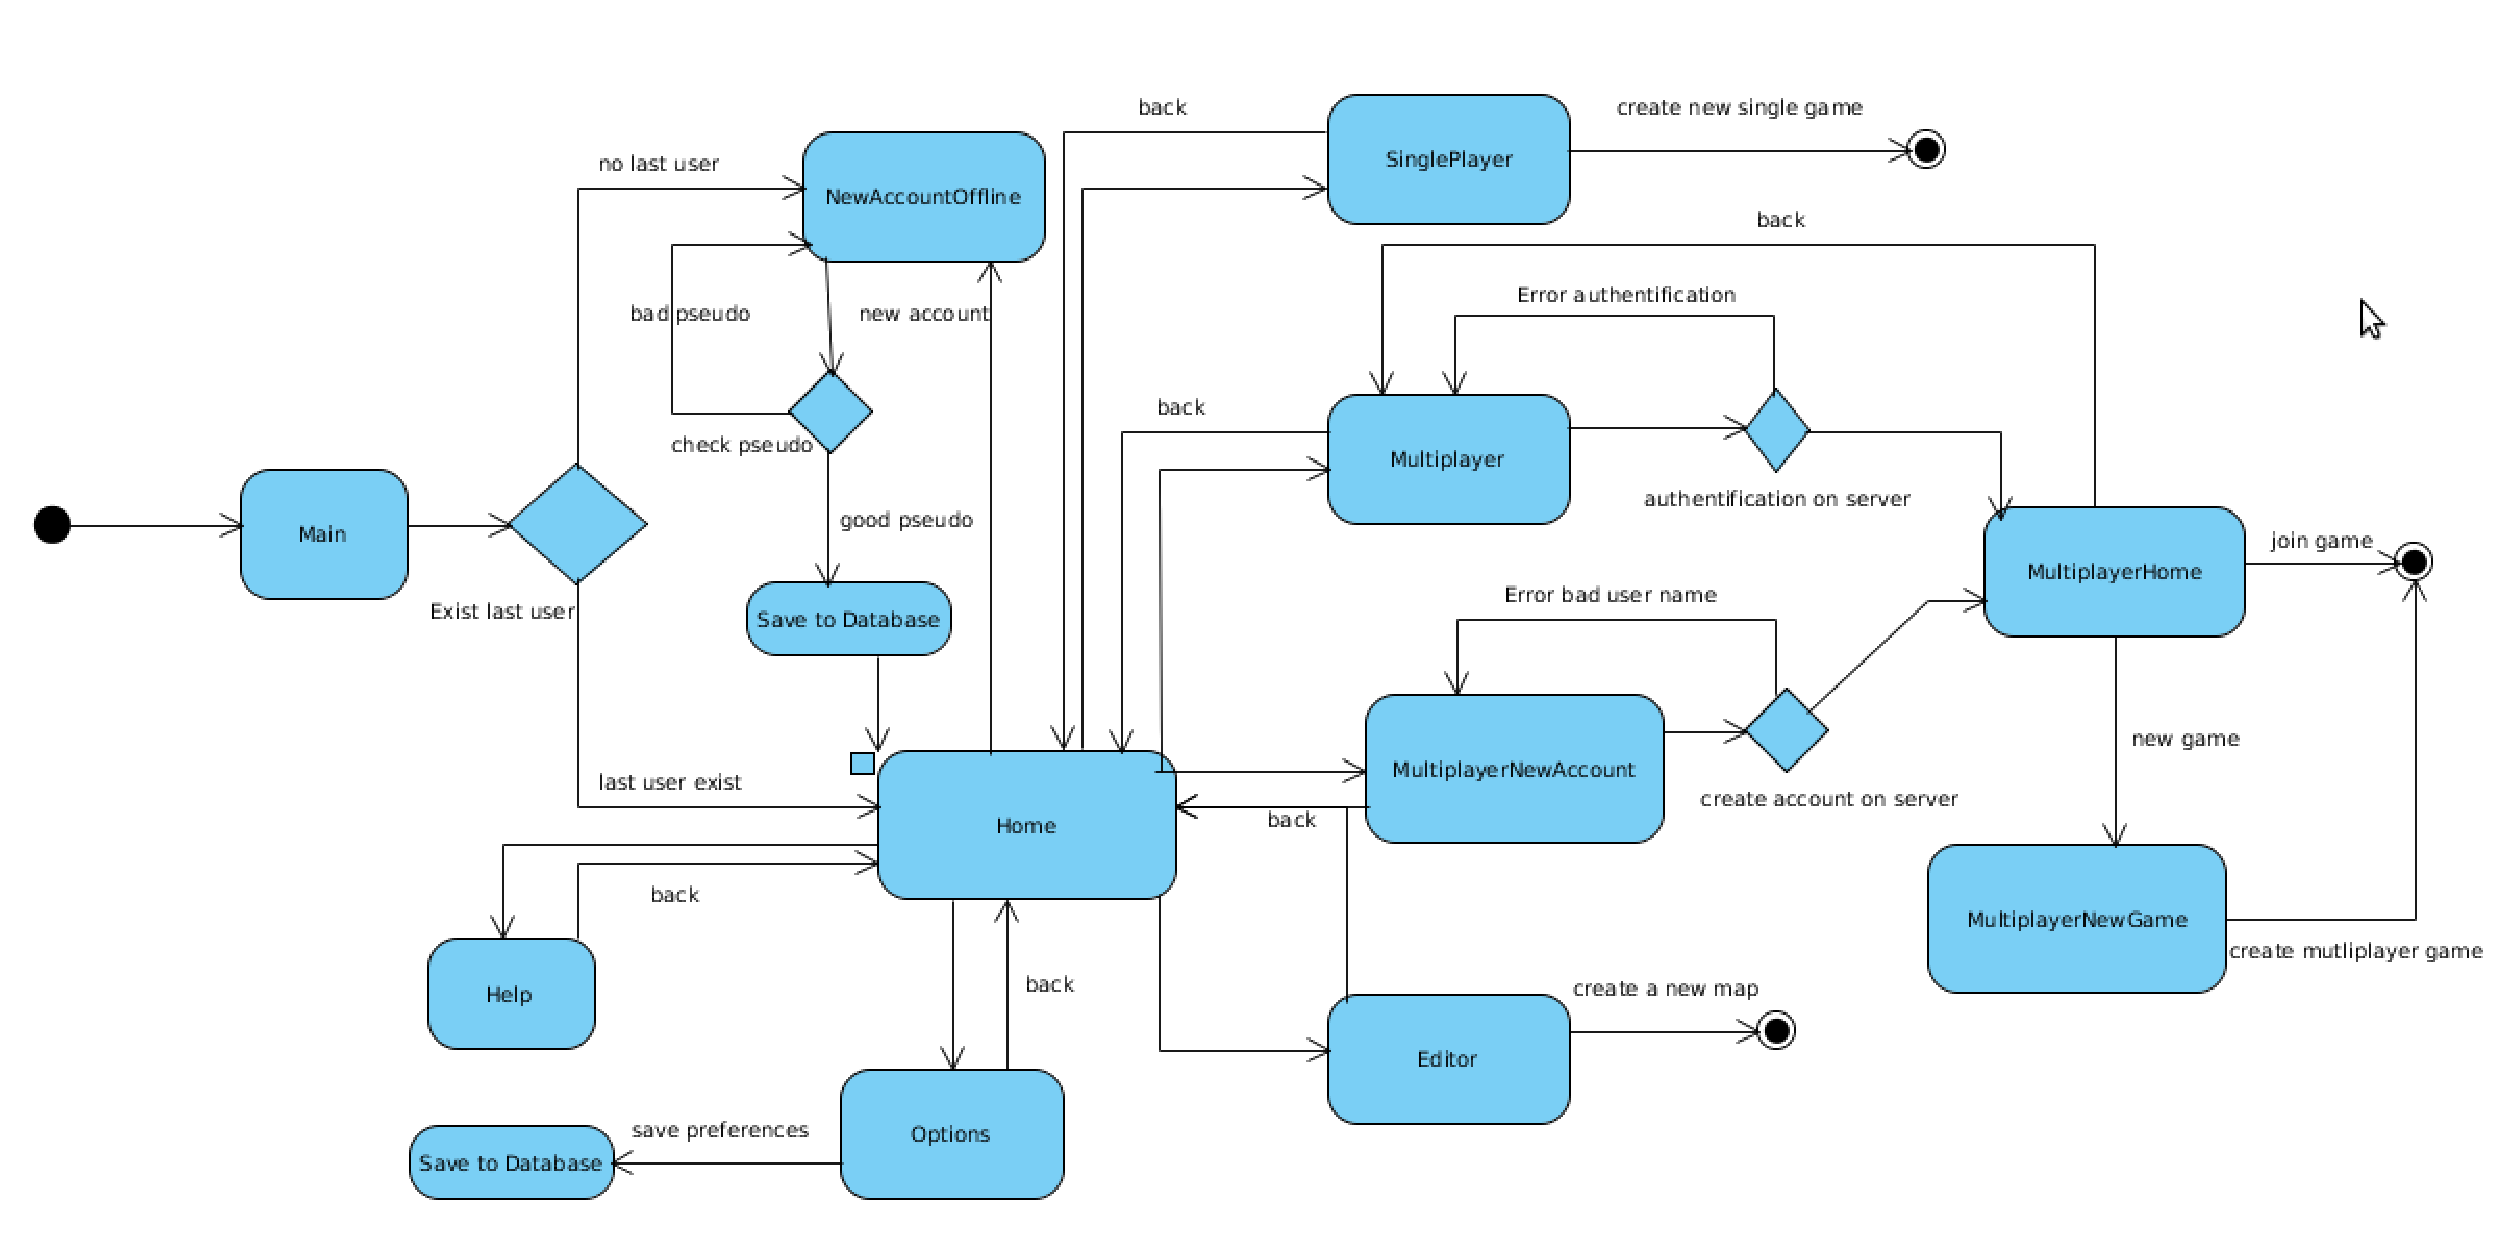
\includegraphics[width=23cm, angle=90]{Analyse/Img/diag_activity.eps}
	\end{center}

	\paragraph{Base de données\\}
			
		Une base de données locale a elle aussi été conçue. Cette dernière a pour
		but de stocker plusieurs types de données.
				
		En effet dès lors qu'un compte local est crée sur le téléphone dans la
		table PlayerAccount, il est possible de conserver ses préférences de joueur
		tel que la couleur du joueur, le pseudonyme ou même ses paramètres de connexion multijoueur. 
		Vous pourrez créer autant de comptes locaux que vous le désirez, et il
		sera possible possible d'éditer ou choisir son compte.
				
		L'application est par ailleur en mesure de conserver
		les valeurs sonores, la langue et même le dernier utilisateur de
		l'application, grâce à un son id qui est clé étrangère dans la table System(lastUser).
				
		De plus l'application sera délivrée avec quelques cartes officielles, mais
		l'utilisateur aura libre droit de créer ses propres cartes de jeu via un
		éditeur. Elles seront alors stockées dans la table Map avec toujours une
		clé étrangère vers l'id de son créateur(owner). \\
				
		\begin{center}
			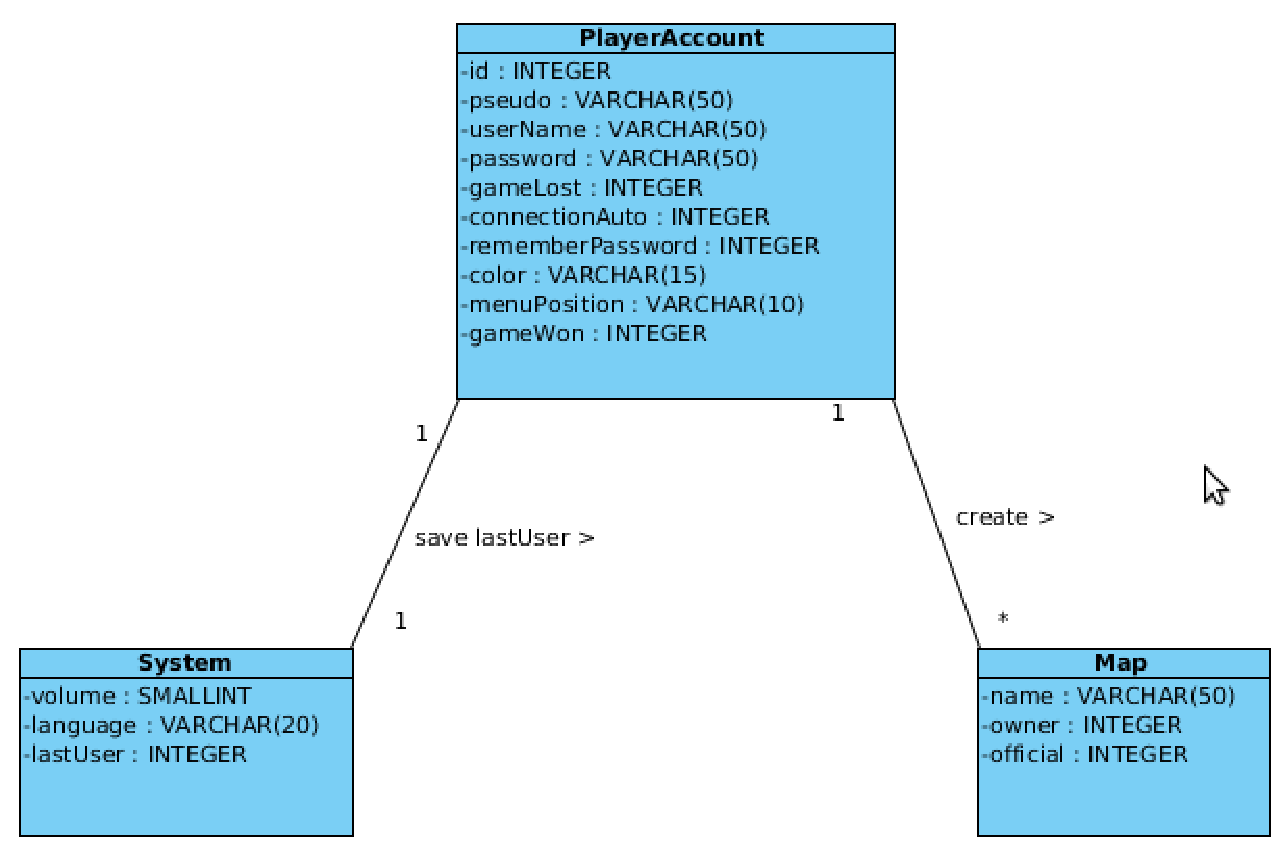
\includegraphics[width=11cm]{Analyse/Img/menu_bdd.eps}
		\end{center}
						
	\paragraph{Scénarios}
			

\subsection{Jeu}
	\begin{itemize}
		\item{Diagramme classe}
		\item{Gameplay}
		\item{Gestion images / tile mapping}
		\item{Images}
		\item{Sons}
	\end{itemize}
			

\subsection{Réseau}
		
	\paragraph{Serveur\\}
			
		Il a été fixé dans le cahier des charges que notre serveur devrait pouvoir
		effectuer plusieurs tâches particulières séparées. Nous avons donc décidé de
		les compartimenter en classes.
			
		Les six éléments situés sur la partie haute du schéma
		ci-dessous(respectivement Inscription, Connection, GamesList, CreateGame,
		ConnectionGame et ManageGame), réprésente les différents tâches demandées.
		Elles sont reliées à une classe nommée contexte, qui leur permettra d'accéder
		aux mêmes données sans qu'il y ait de conflits. La partie basse représente les
		objets qui seront utilisés pour les parties en multijoueurs. Bien évidemment
		ces objets sont très proches de ceux utilisés dans les parties locales.
		
		\begin{center}
			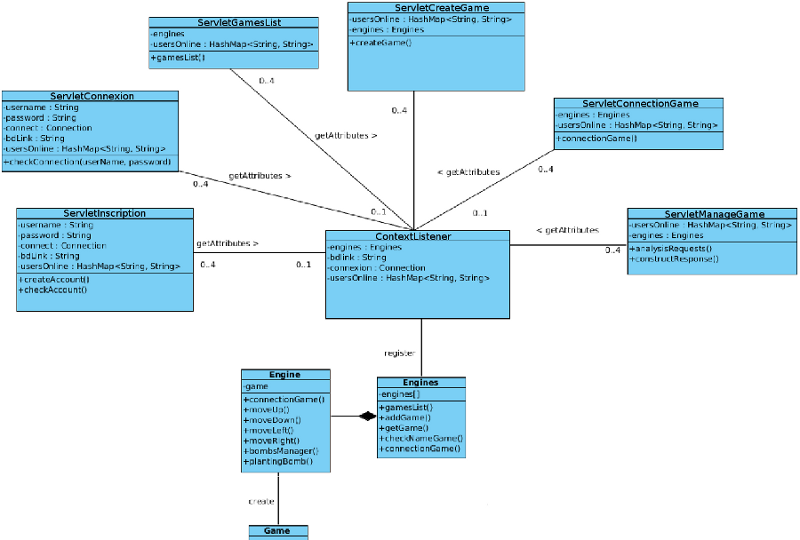
\includegraphics[scale = 0.5]{Analyse/Img/serveur.eps}
		\end{center}
		
	\paragraph{Base de données\\}
		Afin de pouvoir conserver les utilisateurs en lignes ainsi que leurs infos
		personnels pour permettre une authentification, nous avons dû établir une
		base de données sur le serveur. Cette dernière à été pensé comme demandé pour 
		l'enregistrement de comptes. Une unique table nommée Users remplie donc cette
		fonction. Le serveur devra pouvoir y accéder en écriture(inscription) comme
		en lecture(connexion).
			
		Elle ne comportera que deux champs, userName et password.